\documentclass[]{article}
\usepackage{amsmath}
\usepackage{graphicx}
%opening
\title{}
\author{}


\begin{document}

%\maketitle

%\begin{abstract}
%\end{abstract}


Figure \ref{fig:time_evolution} shows the average state as a function of time for two different coupling constants $\mathcal{N}(\bar{\nu}=0.5)$ and  $\mathcal{N}(\bar{\nu}=0.05)$ and different initial conditions $ \mu_{0 n} \sim \mathcal{B} ( \mu; 0.5) $ respectively $ \mu_{0n} \sim\mathcal{B} ( \mu; 0.9 ) $ for $n=1,...,8000$.     %\ref{} . 
 The values of the microscopic parameters are chosen in correspondence with those in the lattice-model \cite{avitabile14}. Each agent is interacting with all other agents. For big coupling constants, the red and green curves show two possible locked-in states. For small coupling constants, the blue curve shows that the mixed state is the unique macroscopic stable equilibrium.

%For a network with 8000 nodes with all-to-all-coupling (all agents in the network interact with all the other agents).
\begin{figure}


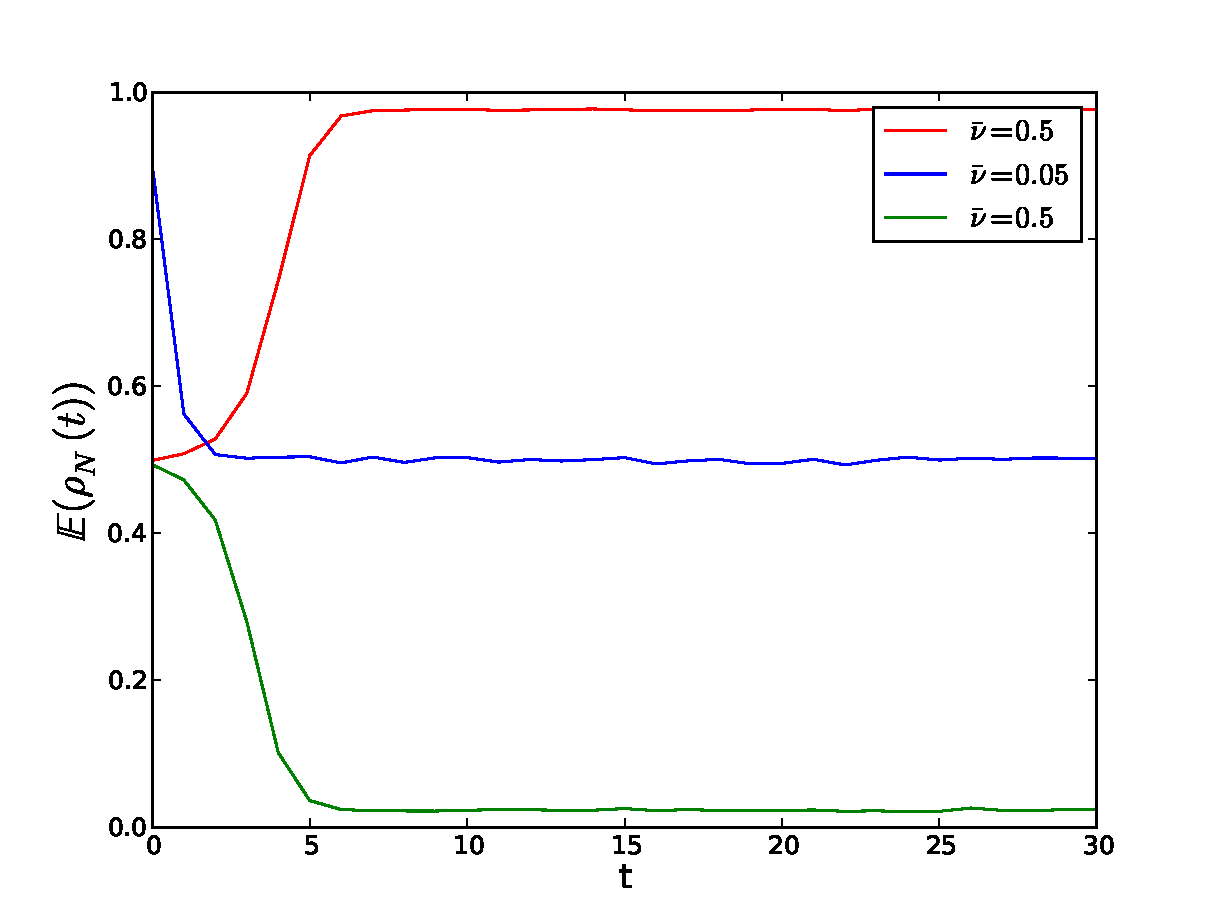
\includegraphics[width=0.9\textwidth]{time_evolution_N_8000.pdf}
\caption{Time evolution of coarse states in a static network with 8000 nodes and all-to-all-coupling.}
\label{fig:time_evolution}
\end{figure}

\bibliographystyle{plain}
\bibliography{biblio.bib}
\end{document}
